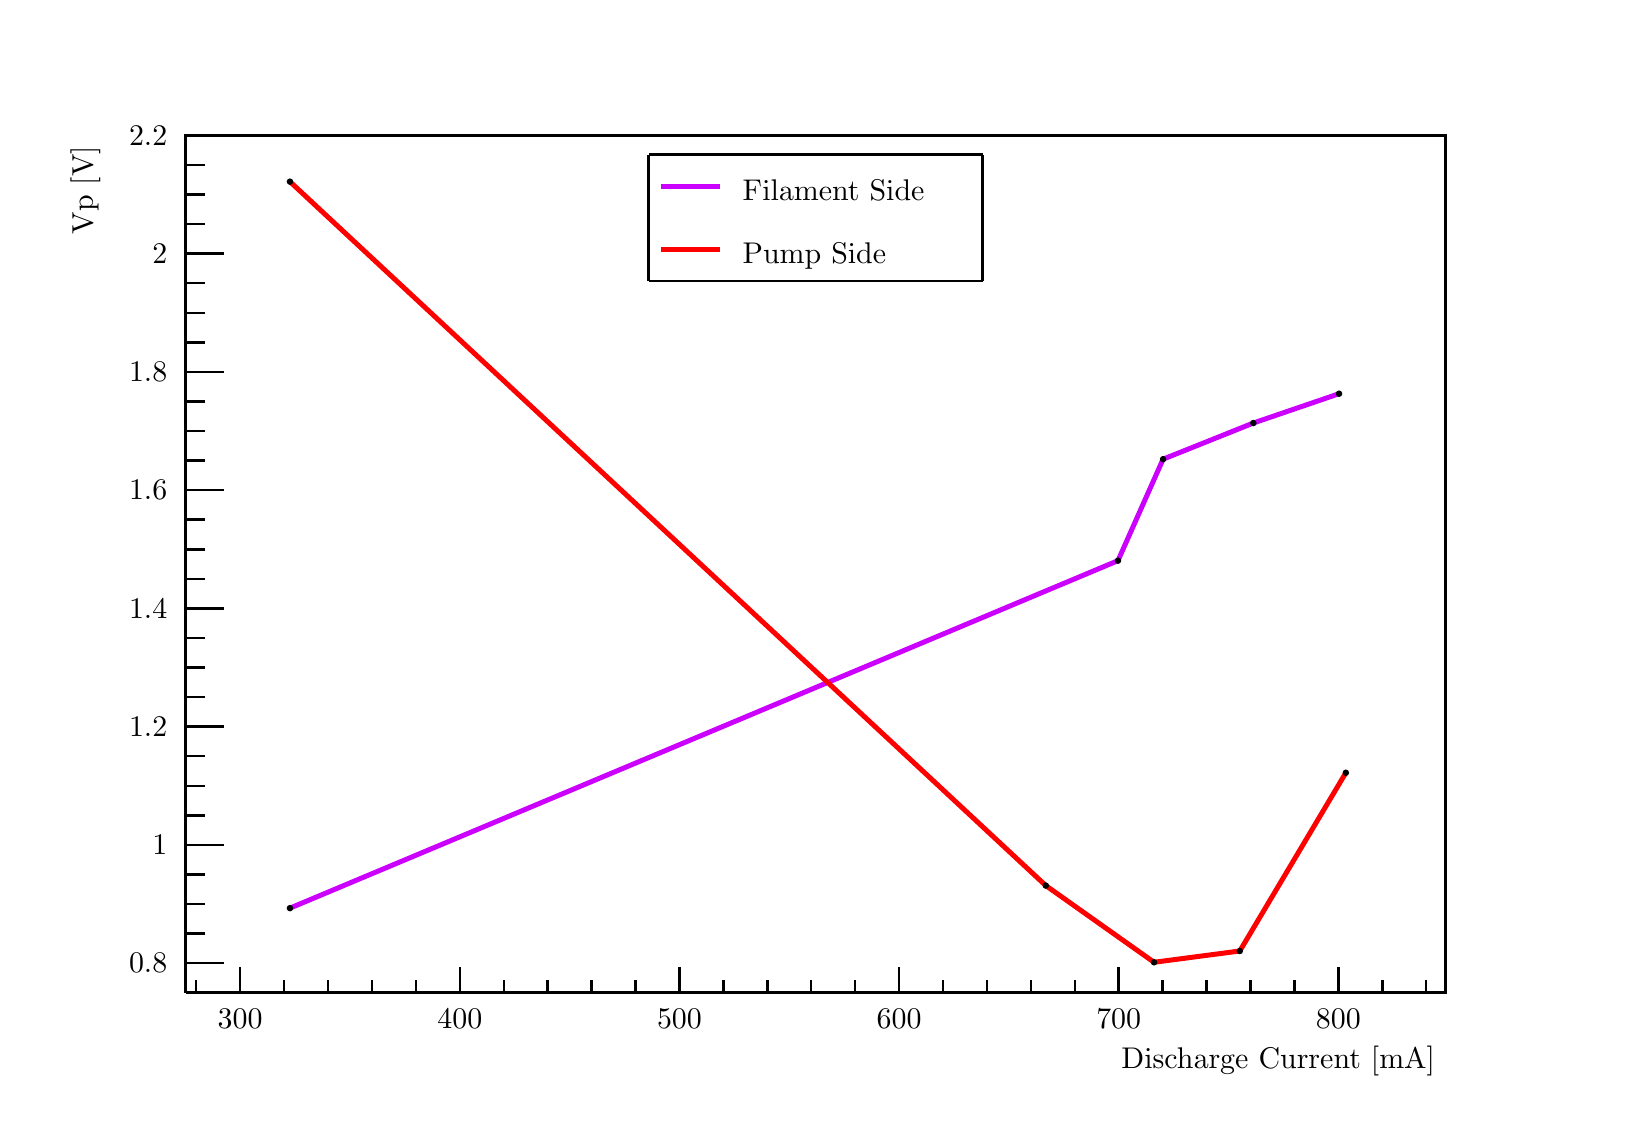
\begin{tikzpicture}
\pgfdeclareplotmark{cross} {
\pgfpathmoveto{\pgfpoint{-0.3\pgfplotmarksize}{\pgfplotmarksize}}
\pgfpathlineto{\pgfpoint{+0.3\pgfplotmarksize}{\pgfplotmarksize}}
\pgfpathlineto{\pgfpoint{+0.3\pgfplotmarksize}{0.3\pgfplotmarksize}}
\pgfpathlineto{\pgfpoint{+1\pgfplotmarksize}{0.3\pgfplotmarksize}}
\pgfpathlineto{\pgfpoint{+1\pgfplotmarksize}{-0.3\pgfplotmarksize}}
\pgfpathlineto{\pgfpoint{+0.3\pgfplotmarksize}{-0.3\pgfplotmarksize}}
\pgfpathlineto{\pgfpoint{+0.3\pgfplotmarksize}{-1.\pgfplotmarksize}}
\pgfpathlineto{\pgfpoint{-0.3\pgfplotmarksize}{-1.\pgfplotmarksize}}
\pgfpathlineto{\pgfpoint{-0.3\pgfplotmarksize}{-0.3\pgfplotmarksize}}
\pgfpathlineto{\pgfpoint{-1.\pgfplotmarksize}{-0.3\pgfplotmarksize}}
\pgfpathlineto{\pgfpoint{-1.\pgfplotmarksize}{0.3\pgfplotmarksize}}
\pgfpathlineto{\pgfpoint{-0.3\pgfplotmarksize}{0.3\pgfplotmarksize}}
\pgfpathclose
\pgfusepathqstroke
}
\pgfdeclareplotmark{cross*} {
\pgfpathmoveto{\pgfpoint{-0.3\pgfplotmarksize}{\pgfplotmarksize}}
\pgfpathlineto{\pgfpoint{+0.3\pgfplotmarksize}{\pgfplotmarksize}}
\pgfpathlineto{\pgfpoint{+0.3\pgfplotmarksize}{0.3\pgfplotmarksize}}
\pgfpathlineto{\pgfpoint{+1\pgfplotmarksize}{0.3\pgfplotmarksize}}
\pgfpathlineto{\pgfpoint{+1\pgfplotmarksize}{-0.3\pgfplotmarksize}}
\pgfpathlineto{\pgfpoint{+0.3\pgfplotmarksize}{-0.3\pgfplotmarksize}}
\pgfpathlineto{\pgfpoint{+0.3\pgfplotmarksize}{-1.\pgfplotmarksize}}
\pgfpathlineto{\pgfpoint{-0.3\pgfplotmarksize}{-1.\pgfplotmarksize}}
\pgfpathlineto{\pgfpoint{-0.3\pgfplotmarksize}{-0.3\pgfplotmarksize}}
\pgfpathlineto{\pgfpoint{-1.\pgfplotmarksize}{-0.3\pgfplotmarksize}}
\pgfpathlineto{\pgfpoint{-1.\pgfplotmarksize}{0.3\pgfplotmarksize}}
\pgfpathlineto{\pgfpoint{-0.3\pgfplotmarksize}{0.3\pgfplotmarksize}}
\pgfpathclose
\pgfusepathqfillstroke
}
\pgfdeclareplotmark{newstar} {
\pgfpathmoveto{\pgfqpoint{0pt}{\pgfplotmarksize}}
\pgfpathlineto{\pgfqpointpolar{44}{0.5\pgfplotmarksize}}
\pgfpathlineto{\pgfqpointpolar{18}{\pgfplotmarksize}}
\pgfpathlineto{\pgfqpointpolar{-20}{0.5\pgfplotmarksize}}
\pgfpathlineto{\pgfqpointpolar{-54}{\pgfplotmarksize}}
\pgfpathlineto{\pgfqpointpolar{-90}{0.5\pgfplotmarksize}}
\pgfpathlineto{\pgfqpointpolar{234}{\pgfplotmarksize}}
\pgfpathlineto{\pgfqpointpolar{198}{0.5\pgfplotmarksize}}
\pgfpathlineto{\pgfqpointpolar{162}{\pgfplotmarksize}}
\pgfpathlineto{\pgfqpointpolar{134}{0.5\pgfplotmarksize}}
\pgfpathclose
\pgfusepathqstroke
}
\pgfdeclareplotmark{newstar*} {
\pgfpathmoveto{\pgfqpoint{0pt}{\pgfplotmarksize}}
\pgfpathlineto{\pgfqpointpolar{44}{0.5\pgfplotmarksize}}
\pgfpathlineto{\pgfqpointpolar{18}{\pgfplotmarksize}}
\pgfpathlineto{\pgfqpointpolar{-20}{0.5\pgfplotmarksize}}
\pgfpathlineto{\pgfqpointpolar{-54}{\pgfplotmarksize}}
\pgfpathlineto{\pgfqpointpolar{-90}{0.5\pgfplotmarksize}}
\pgfpathlineto{\pgfqpointpolar{234}{\pgfplotmarksize}}
\pgfpathlineto{\pgfqpointpolar{198}{0.5\pgfplotmarksize}}
\pgfpathlineto{\pgfqpointpolar{162}{\pgfplotmarksize}}
\pgfpathlineto{\pgfqpointpolar{134}{0.5\pgfplotmarksize}}
\pgfpathclose
\pgfusepathqfillstroke
}
\definecolor{c}{rgb}{1,1,1};
\draw [color=c, fill=c] (0,0) rectangle (20,13.6103);
\draw [color=c, fill=c] (2,1.36103) rectangle (18,12.2493);
\definecolor{c}{rgb}{0,0,0};
\draw [c,line width=0.9] (2,1.36103) -- (2,12.2493) -- (18,12.2493) -- (18,1.36103) -- (2,1.36103);
\definecolor{c}{rgb}{1,1,1};
\draw [color=c, fill=c] (2,1.36103) rectangle (18,12.2493);
\definecolor{c}{rgb}{0,0,0};
\draw [c,line width=0.9] (2,1.36103) -- (2,12.2493) -- (18,12.2493) -- (18,1.36103) -- (2,1.36103);
\draw [c,line width=0.9] (2,1.36103) -- (18,1.36103);
\draw [c,line width=0.9] (2.69177,1.68768) -- (2.69177,1.36103);
\draw [c,line width=0.9] (3.24965,1.52436) -- (3.24965,1.36103);
\draw [c,line width=0.9] (3.80753,1.52436) -- (3.80753,1.36103);
\draw [c,line width=0.9] (4.36541,1.52436) -- (4.36541,1.36103);
\draw [c,line width=0.9] (4.92329,1.52436) -- (4.92329,1.36103);
\draw [c,line width=0.9] (5.48117,1.68768) -- (5.48117,1.36103);
\draw [c,line width=0.9] (6.03905,1.52436) -- (6.03905,1.36103);
\draw [c,line width=0.9] (6.59693,1.52436) -- (6.59693,1.36103);
\draw [c,line width=0.9] (7.15481,1.52436) -- (7.15481,1.36103);
\draw [c,line width=0.9] (7.71269,1.52436) -- (7.71269,1.36103);
\draw [c,line width=0.9] (8.27057,1.68768) -- (8.27057,1.36103);
\draw [c,line width=0.9] (8.82845,1.52436) -- (8.82845,1.36103);
\draw [c,line width=0.9] (9.38633,1.52436) -- (9.38633,1.36103);
\draw [c,line width=0.9] (9.94421,1.52436) -- (9.94421,1.36103);
\draw [c,line width=0.9] (10.5021,1.52436) -- (10.5021,1.36103);
\draw [c,line width=0.9] (11.06,1.68768) -- (11.06,1.36103);
\draw [c,line width=0.9] (11.6179,1.52436) -- (11.6179,1.36103);
\draw [c,line width=0.9] (12.1757,1.52436) -- (12.1757,1.36103);
\draw [c,line width=0.9] (12.7336,1.52436) -- (12.7336,1.36103);
\draw [c,line width=0.9] (13.2915,1.52436) -- (13.2915,1.36103);
\draw [c,line width=0.9] (13.8494,1.68768) -- (13.8494,1.36103);
\draw [c,line width=0.9] (14.4073,1.52436) -- (14.4073,1.36103);
\draw [c,line width=0.9] (14.9651,1.52436) -- (14.9651,1.36103);
\draw [c,line width=0.9] (15.523,1.52436) -- (15.523,1.36103);
\draw [c,line width=0.9] (16.0809,1.52436) -- (16.0809,1.36103);
\draw [c,line width=0.9] (16.6388,1.68768) -- (16.6388,1.36103);
\draw [c,line width=0.9] (2.69177,1.68768) -- (2.69177,1.36103);
\draw [c,line width=0.9] (2.13389,1.52436) -- (2.13389,1.36103);
\draw [c,line width=0.9] (16.6388,1.68768) -- (16.6388,1.36103);
\draw [c,line width=0.9] (17.1967,1.52436) -- (17.1967,1.36103);
\draw [c,line width=0.9] (17.7545,1.52436) -- (17.7545,1.36103);
\draw [anchor=base] (2.69177,0.911891) node[scale=1.08185, color=c, rotate=0]{300};
\draw [anchor=base] (5.48117,0.911891) node[scale=1.08185, color=c, rotate=0]{400};
\draw [anchor=base] (8.27057,0.911891) node[scale=1.08185, color=c, rotate=0]{500};
\draw [anchor=base] (11.06,0.911891) node[scale=1.08185, color=c, rotate=0]{600};
\draw [anchor=base] (13.8494,0.911891) node[scale=1.08185, color=c, rotate=0]{700};
\draw [anchor=base] (16.6388,0.911891) node[scale=1.08185, color=c, rotate=0]{800};
\draw [anchor= east] (18,0.499771) node[scale=1.08185, color=c, rotate=0]{Discharge Current [mA]};
\draw [c,line width=0.9] (2,1.36103) -- (2,12.2493);
\draw [c,line width=0.9] (2.48,1.73649) -- (2,1.73649);
\draw [c,line width=0.9] (2.24,2.11195) -- (2,2.11195);
\draw [c,line width=0.9] (2.24,2.4874) -- (2,2.4874);
\draw [c,line width=0.9] (2.24,2.86286) -- (2,2.86286);
\draw [c,line width=0.9] (2.48,3.23832) -- (2,3.23832);
\draw [c,line width=0.9] (2.24,3.61377) -- (2,3.61377);
\draw [c,line width=0.9] (2.24,3.98923) -- (2,3.98923);
\draw [c,line width=0.9] (2.24,4.36469) -- (2,4.36469);
\draw [c,line width=0.9] (2.48,4.74014) -- (2,4.74014);
\draw [c,line width=0.9] (2.24,5.1156) -- (2,5.1156);
\draw [c,line width=0.9] (2.24,5.49106) -- (2,5.49106);
\draw [c,line width=0.9] (2.24,5.86652) -- (2,5.86652);
\draw [c,line width=0.9] (2.48,6.24197) -- (2,6.24197);
\draw [c,line width=0.9] (2.24,6.61743) -- (2,6.61743);
\draw [c,line width=0.9] (2.24,6.99289) -- (2,6.99289);
\draw [c,line width=0.9] (2.24,7.36834) -- (2,7.36834);
\draw [c,line width=0.9] (2.48,7.7438) -- (2,7.7438);
\draw [c,line width=0.9] (2.24,8.11926) -- (2,8.11926);
\draw [c,line width=0.9] (2.24,8.49471) -- (2,8.49471);
\draw [c,line width=0.9] (2.24,8.87017) -- (2,8.87017);
\draw [c,line width=0.9] (2.48,9.24563) -- (2,9.24563);
\draw [c,line width=0.9] (2.24,9.62109) -- (2,9.62109);
\draw [c,line width=0.9] (2.24,9.99654) -- (2,9.99654);
\draw [c,line width=0.9] (2.24,10.372) -- (2,10.372);
\draw [c,line width=0.9] (2.48,10.7475) -- (2,10.7475);
\draw [c,line width=0.9] (2.24,11.1229) -- (2,11.1229);
\draw [c,line width=0.9] (2.24,11.4984) -- (2,11.4984);
\draw [c,line width=0.9] (2.24,11.8738) -- (2,11.8738);
\draw [c,line width=0.9] (2.48,12.2493) -- (2,12.2493);
\draw [c,line width=0.9] (2.48,1.73649) -- (2,1.73649);
\draw [c,line width=0.9] (2.24,1.36103) -- (2,1.36103);
\draw [anchor= east] (1.9,1.73649) node[scale=1.08185, color=c, rotate=0]{0.8};
\draw [anchor= east] (1.9,3.23832) node[scale=1.08185, color=c, rotate=0]{1};
\draw [anchor= east] (1.9,4.74014) node[scale=1.08185, color=c, rotate=0]{1.2};
\draw [anchor= east] (1.9,6.24197) node[scale=1.08185, color=c, rotate=0]{1.4};
\draw [anchor= east] (1.9,7.7438) node[scale=1.08185, color=c, rotate=0]{1.6};
\draw [anchor= east] (1.9,9.24563) node[scale=1.08185, color=c, rotate=0]{1.8};
\draw [anchor= east] (1.9,10.7475) node[scale=1.08185, color=c, rotate=0]{2};
\draw [anchor= east] (1.9,12.2493) node[scale=1.08185, color=c, rotate=0]{2.2};
\draw [anchor= east] (0.726934,12.2493) node[scale=1.08185, color=c, rotate=90]{Vp [V]};
\definecolor{c}{rgb}{0.8,0,1};
\draw [c,line width=1.8] (3.32378,2.43553) -- (13.8395,6.84814) -- (14.4126,8.13754) -- (15.5587,8.59599) -- (16.6476,8.96848);
\definecolor{c}{rgb}{0,0,0};
\foreach \P in {(3.32378,2.43553), (13.8395,6.84814), (14.4126,8.13754), (15.5587,8.59599), (16.6476,8.96848)}{\draw[mark options={color=c,fill=c},mark size=0.960961pt,mark=*] plot coordinates {\P};}
\definecolor{c}{rgb}{1,0,0};
\draw [c,line width=1.8] (3.32378,11.6619) -- (12.9226,2.72206) -- (14.298,1.74785) -- (15.3868,1.89112) -- (16.7335,4.15473);
\definecolor{c}{rgb}{0,0,0};
\foreach \P in {(3.32378,11.6619), (12.9226,2.72206), (14.298,1.74785), (15.3868,1.89112), (16.7335,4.15473)}{\draw[mark options={color=c,fill=c},mark size=0.960961pt,mark=*] plot coordinates {\P};}
\definecolor{c}{rgb}{1,1,1};
\draw [color=c, fill=c] (7.87966,10.4011) rectangle (12.1203,12.0057);
\definecolor{c}{rgb}{0,0,0};
\draw [c,line width=0.9] (7.87966,10.4011) -- (12.1203,10.4011);
\draw [c,line width=0.9] (12.1203,10.4011) -- (12.1203,12.0057);
\draw [c,line width=0.9] (12.1203,12.0057) -- (7.87966,12.0057);
\draw [c,line width=0.9] (7.87966,12.0057) -- (7.87966,10.4011);
\draw [anchor=base west] (8.93983,11.4241) node[scale=1.08185, color=c, rotate=0]{Filament Side};
\definecolor{c}{rgb}{0.8,0,1};
\draw [c,line width=1.8] (8.03868,11.6046) -- (8.7808,11.6046);
\definecolor{c}{rgb}{0,0,0};
\draw [anchor=base west] (8.93983,10.6218) node[scale=1.08185, color=c, rotate=0]{Pump Side};
\definecolor{c}{rgb}{1,0,0};
\draw [c,line width=1.8] (8.03868,10.8023) -- (8.7808,10.8023);
\end{tikzpicture}
